% !TeX root = ../../Book1.tex
% 纲要标题：### 8.5 模型、形变与刚性的界线
% 纲要位置：几何学计划纲要.md，第 453 行。
% 正文状态：初稿；尚未正式审核。

% 纲要内容开始
% 
% * 球面、圆柱和旋转曲面的核验
% * 平面与圆柱的局部等距
% * 一阶、局部和整体刚性问题的区分
% 
% ---
% 
% 纲要内容结束

\section{模型、形变与刚性的界线}
\label{g1:sec:0805}

曲面基本定理需要同时给定 \(I\) 和 \(II\)。如果只给 \(I\)，内在曲率虽然已经确定，两个主曲率及曲面在空间中的形状却还可能变化。本节把这种自由算在几个熟悉模型上，再区分三个常被混在一起的问题：一个变动在一阶上是否保持度量，是否存在真实的等距形变，以及局部构造能否在整张曲面上成立。

\subsection{球面、圆柱和旋转曲面的核验}
\label{g1:subsec:0805:01}

\begin{example}[球面与法向的符号]\label{g1:exm:sphere-two-forms}
	半径 \(R>0\) 的球面去掉两极后，可在经度的局部区间中用
	\[
		X(s,\theta)=\bigl(R\sin(s/R)\cos\theta,\ R\sin(s/R)\sin\theta,\ R\cos(s/R)\bigr),
		\quad 0<s<\pi R
	\]
	参数化。直接求导得到
	\[
		I=\mathrm{d}s^2+R^2\sin^2(s/R)\,\mathrm{d}\theta^2,\qquad
		n=\frac{X}{R}=\frac{X_s\times X_\theta}{\|X_s\times X_\theta\|}.
	\]
	因为 \(\mathrm{d}n=\mathrm{d}X/R\)，本书约定 \(S=-\mathrm{d}n\) 给出 \(S=-R^{-1}\operatorname{id}\)，所以
	\[
		II=-R^{-1}I,\qquad k_1=k_2=-R^{-1},\qquad H=-R^{-1},\qquad K=R^{-2}.
	\]
	因此标准球面仍有正的 Gauss 曲率；外向法向下主曲率为负，与 \(S=-\mathrm{d}n\) 一致。反向选择法向时 \(II,H,k_1,k_2\) 改号，\(I,K\) 不变。参数在两极退化，因为 \(X_\theta=0\)，但球面本身在那里可以改用图像坐标，没有几何奇点。
\end{example}

\begin{example}[圆柱的两个方向]\label{g1:exm:cylinder-two-forms}
	取
	\[
		C(u,v)=\bigl(R\cos(u/R),R\sin(u/R),v\bigr),\qquad R>0.
	\]
	有 \(C_u=(-\sin(u/R),\cos(u/R),0)\)、\(C_v=(0,0,1)\)，两者单位且正交。外向法向 \(n=(\cos(u/R),\sin(u/R),0)\) 等于 \(C_u\times C_v\)，而
	\[
		n_u=R^{-1}C_u,\qquad n_v=0.
	\]
	故
	\[
		I=\mathrm{d}u^2+\mathrm{d}v^2,\qquad II=-R^{-1}\mathrm{d}u^2,\qquad
		k_1=-R^{-1},\quad k_2=0,\quad H=-\frac1{2R},\quad K=0.
	\]
	圆周方向发生弯曲，母线方向没有法向弯曲。这里有一个零主曲率并不表示整张曲面是平面，也不表示参数不正则。
\end{example}

这两例都可由旋转曲面的统一公式找回。取光滑单位速率平面曲线 \((r(s),z(s))\)，假设 \(r>0\) 且 \(r'^2+z'^2=1\)，绕 \(z\) 轴旋转：
\[
	X(s,\theta)=(r(s)\cos\theta,r(s)\sin\theta,z(s)).
\]
弧长条件只作用于母线；\(\theta\) 方向的长度因子仍为 \(r\)。

\begin{proposition}[旋转曲面的基本形式]\label{g1:prop:revolution-two-forms}
	在上述光滑单位速率母线、\(r>0\) 及局部角参数条件下，选择法向
	\[
		n=(-z'\cos\theta,-z'\sin\theta,r'),
	\]
	则
	\[
		I=\mathrm{d}s^2+r^2\mathrm{d}\theta^2,\qquad
		II=(r'z''-z'r'')\,\mathrm{d}s^2+rz'\,\mathrm{d}\theta^2.
	\]
	子午线和纬线方向为主方向，主曲率及 Gauss 曲率为
	\begin{equation}\label{g1:eq:revolution-curvatures}
		k_s=r'z''-z'r'',\qquad k_\theta=\frac{z'}r,\qquad
		K=-\frac{r''}r,\qquad H=\frac12\left(r'z''-z'r''+\frac{z'}r\right).
	\end{equation}
	在脐点，这两方向仍是主方向，但不再是仅有的主方向。
\end{proposition}

\begin{proof}
	计算 \(X_s,X_\theta\) 得到 \(\|X_s\|=1\)、\(\|X_\theta\|=r\)、\(\langle X_s,X_\theta\rangle=0\)，且 \(X_s\times X_\theta=rn\)。二阶导数与 \(n\) 的内积分别是
	\[
		\langle X_{ss},n\rangle=-z'r''+r'z'',\qquad
		\langle X_{s\theta},n\rangle=0,\qquad
		\langle X_{\theta\theta},n\rangle=rz'.
	\]
	因此 \(I,II\) 都对角，形算子的两个特征值是相应对角项之比。最后，由单位速率条件求导得 \(r'r''+z'z''=0\)，从而
	\[
		z'(r'z''-z'r'')=-r'^2r''-z'^2r''=-r'',
	\]
	即得 \(K=-r''/r\)。此推导没有除以 \(z'\)，故 \(z'=0\) 的点也包括在内。
\end{proof}

令 \(r=R\sin(s/R),z=R\cos(s/R)\)，就得到外向球面的两个负主曲率。令 \(r=R,z=s\)，则上面指定的法向朝向圆柱轴线，因而 \(k_\theta=1/R\)；它与前一例的负号差别完全来自法向，不能直接混用。对圆锥的去顶点部分，取 \(r=as,z=bs\)，其中 \(s>0,a>0,a^2+b^2=1\)，可得 \(K=0\)。\(r=0\) 的顶点不属于命题的适用区域，零曲率公式不能被延伸为顶点正则性的证明。

\begin{example}[一个非平面的负曲率模型]\label{g1:exm:catenoid-curvatures}
	取 \(r(s)=\sqrt{a^2+s^2}\)、\(z(s)=a\,\operatorname{arsinh}(s/a)\)，其中 \(a>0\)。这里 \(\operatorname{arsinh}\) 是双曲正弦的反函数，导数为 \(1/\sqrt{1+t^2}\)。计算得
	\[
		r'=\frac{s}{r},\quad z'=\frac ar,\quad
		r''=\frac{a^2}{r^3},\quad z''=-\frac{as}{r^3}.
	\]
	因此母线确实单位速率，而旋转曲面的 \(k_s=-a/r^2\)、\(k_\theta=a/r^2\)，故 \(H=0\)、\(K=-a^2/r^4<0\)。这是\term[xuanlianmian]{悬链面}[catenoid]的一个弧长参数表示。平均曲率为零表示两个带符号主曲率相互抵消，绝不是两个主曲率都为零。
\end{example}

\subsection{平面与圆柱的局部等距}
\label{g1:subsec:0805:02}

平面 \(P(u,v)=(u,v,0)\) 与圆柱参数 \(C(u,v)\) 的第一基本形式都为 \(\mathrm{d}u^2+\mathrm{d}v^2\)。在宽度小于 \(2\pi R\) 的开条带上，\(C\) 单射，故对应 \(P(u,v)\mapsto C(u,v)\) 是局部曲面之间的等距。由\cref{g1:prop:local-isometry-length}，任意纸上曲线的长度以及相交角度都保持；这正是“无拉伸卷起”的数学含义。

\ProseParagraphBreak

它不可能由空间刚性运动得到：平面的第二基本形式恒为零，而圆柱的第二基本形式不为零；刚性运动保持第二基本形式（同时推送所选法向），反射至多因法向约定带来整体改号，也不能把零变成非零。第一基本形式的相同因此不足以触发上一节的曲面唯一性结论。

\begin{example}[从平面连续卷起]\label{g1:exm:plane-cylinder-bending}
	在固定有界矩形 \(U=(-a,a)\times(-b,b)\) 上定义
	\[
		X_t(u,v)=
		\begin{cases}
			\bigl(\sin(tu)/t,\ v,\ (1-\cos(tu))/t\bigr),&t\ne0,\\
			(u,v,0),&t=0.
		\end{cases}
	\]
	函数 \(\sin(tu)/t=\int_0^u\cos(t\xi)\,\mathrm{d}\xi\)、\((1-\cos(tu))/t=\int_0^u\sin(t\xi)\,\mathrm{d}\xi\) 表明 \(X_t\) 对 \((t,u,v)\) 光滑，并无真实的 \(t=0\) 奇点。因为
	\[
		(X_t)_u=(\cos(tu),0,\sin(tu)),\qquad (X_t)_v=(0,1,0),
	\]
	全部 \(t\) 对应的第一基本形式都为 \(\mathrm{d}u^2+\mathrm{d}v^2\)。取 \(n_t=(-\sin(tu),0,\cos(tu))\)，则 \(II_t=t\,\mathrm{d}u^2\)。当 \(|t|a<\pi/2\) 时第一坐标对 \(u\) 严格递增，故每个 \(X_t\) 还是嵌入。这个例子既给出真实的局部等距形变，又清楚显示被改变的数据是第二基本形式。
\end{example}

\cref{g1:fig:plane-cylinder-bending}画出同一参数网格在 \(t=0\) 与 \(t=1\) 时的样子。网格线在图纸上的投影长度可以不同；被保持的是曲面自身的 \(I\)，并非观看图像时的平面投影距离。

% !TeX root = ../Book1.tex
\begin{figure}[htbp]
	\centering
	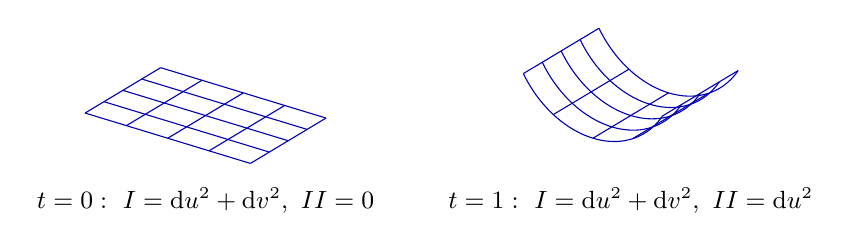
\begin{tikzpicture}[x={(1.05cm,-0.32cm)},y={(0.6cm,0.36cm)},z={(0cm,1.2cm)},font=\small]
		\begin{scope}[xshift=-2.8cm]
			\foreach \a in {-1,-0.5,0,0.5,1}{\draw[blue!70!black] (\a,-0.8,0)--(\a,0.8,0);}
			\foreach \b in {-0.8,-0.4,0,0.4,0.8}{\draw[blue!70!black] (-1,\b,0)--(1,\b,0);}
			\node at (0,0,-0.9) {\(t=0:\ I=\mathrm{d}u^2+\mathrm{d}v^2,\ II=0\)};
		\end{scope}
		\begin{scope}[xshift=2.6cm]
			\foreach \a in {-1,-0.5,0,0.5,1}{\draw[blue!70!black] ({sin(deg(\a))},-0.8,{1-cos(deg(\a))})--({sin(deg(\a))},0.8,{1-cos(deg(\a))});}
			\foreach \b in {-0.8,-0.4,0,0.4,0.8}{\draw[blue!70!black,domain=-1:1,samples=41,variable=\a] plot ({sin(deg(\a))},\b,{1-cos(deg(\a))});}
			\node at (0,0,-0.9) {\(t=1:\ I=\mathrm{d}u^2+\mathrm{d}v^2,\ II=\mathrm{d}u^2\)};
		\end{scope}
	\end{tikzpicture}
	\caption[平面卷成圆柱片]{同一参数网格的等距形变。两图的第一基本形式相同；弯曲后沿 \(u\) 方向的法向随位置改变，第二基本形式随之改变。图中采用例中的法向约定。}
	\label{g1:fig:plane-cylinder-bending}
\end{figure}


如果在整个参数平面上使用 \(C\)，则 \(C(u+2\pi R,v)=C(u,v)\)。它仍逐点保持度量，却不再单射，因而不是平面到整张圆柱的等距。更强地，平面与整张圆柱之间不存在任何整体微分同胚：平面可收缩，而圆柱投影到圆周的映射与固定高度的圆周包含互为收缩关系，绕轴一周的道路不可能收缩成点。后一断言可直接由\cref{g1:thm:circle-fundamental}中 \(\pi_1(S^1)\cong\mathbb Z\) 及投影、包含的复合为恒等得到。这个拓扑障碍与局部度量计算并不矛盾。

\subsection{一阶、局部和整体刚性问题的区分}
\label{g1:subsec:0805:03}

“刚性”必须说明保持什么、在哪个区域比较以及是否允许改变参数。曲面基本定理的唯一性固定了参数域上的两种形式：若两个浸入的 \(I,II\) 相同，才比较它们是否由一个固定的空间刚性运动联系。若给定一个参数对应 \(\phi\)，应先将第二个浸入换成 \(\widetilde X\circ\phi\)，再逐项比较两种形式。

\begin{definition}[无穷小等距变动]\label{g1:def:infinitesimal-bending}
	设 \(X:U\rightarrow\mathbb R^3\) 为光滑浸入，\(V:U\rightarrow\mathbb R^3\) 为沿 \(X\) 的光滑向量场。若
	\begin{equation}\label{g1:eq:infinitesimal-bending}
		\langle\partial_iV,X_j\rangle+\langle X_i,\partial_jV\rangle=0,\qquad i,j=1,2,
	\end{equation}
	称 \(V\) 为一个\term[wuqiongxiaodengjubiandong]{无穷小等距变动}[infinitesimal bending]。若 \(V=a+\Omega X\)，其中 \(a\in\mathbb R^3\) 固定、\(\Omega\) 为固定斜对称矩阵，称其为刚性运动产生的变动。
\end{definition}

几何上 \(V(q)\) 是曲面点最初的移动速度。若光滑族 \(X_t\) 满足 \(X_0=X\)，则对 \(g_{ij}(t)=\langle(X_t)_i,(X_t)_j\rangle\) 求 \(t\) 导数，正好得到\eqref{g1:eq:infinitesimal-bending}，其中 \(V=\partial_tX_t|_{t=0}\)。因此真正的等距形变一定产生无穷小等距变动。斜对称矩阵给出
\[
	\langle\Omega X_i,X_j\rangle+\langle X_i,\Omega X_j\rangle=0,
\]
所以刚性运动产生的变动总满足这个线性方程。

\begin{example}[一阶条件并不足够]\label{g1:exm:nonintegrable-plane-bending}
	对平面 \(X(u,v)=(u,v,0)\)，任意光滑函数 \(f\) 都给出 \(V=f(u,v)(0,0,1)\)，并满足\eqref{g1:eq:infinitesimal-bending}，因为 \(\partial_iV\) 总与平面垂直。它不一定来自真正的等距形变。取 \(f=u^2+v^2\)，假设有对 \((t,u,v)\) 光滑的浸入族 \(X_t\)，使 \(X_0=X\)、\(\partial_tX_t|_0=V\)，且 \(I_t=\mathrm{d}u^2+\mathrm{d}v^2\)。取由参数定向决定的法向 \(n_t\)。因为 \(X_{ij}|_{t=0}=0\)，
	\[
		h_{ij}(0)=0,\qquad
		\left.\partial_t h_{ij}(t)\right|_0
		=\langle\partial_i\partial_jV,(0,0,1)\rangle=f_{ij}.
	\]
	因此在任一固定参数点有 \(h(t)=2tI_2+O(t^2)\)，从而 \(\det h(t)=4t^2+O(t^3)\)。可是固定的平面度量具有 \(K=0\)，由\cref{g1:thm:gauss-equation}必须有 \(\det h(t)=K\det g=0\)，矛盾。这里一阶约束全满足，二阶相容性却阻止了真实形变。
\end{example}

相比之下，\cref{g1:exm:plane-cylinder-bending}在 \(t=0\) 的变动为 \(V=(u^2/2)(0,0,1)\)，它确实来自整个等距族；其二阶导数矩阵的行列式为零。这个比较只说明上述必要障碍在后一例中消失，不能反过来把“行列式为零”未经证明地宣布为任意形变都可积分的充分条件。

\begin{proposition}[两种形式相同的整体唯一性]\label{g1:prop:surface-global-uniqueness}
	设 \(U\subseteq\mathbb R^2\) 为连通开集，\(X,\widetilde X:U\rightarrow\mathbb R^3\) 为光滑浸入，均取参数定向的单位法向。若两者在同一参数下具有相同的第一、第二基本形式，则存在一个固定 \(Q\in \operatorname{SO}(3)\) 和 \(a\in\mathbb R^3\)，使 \(\widetilde X=QX+a\) 在整个 \(U\) 上成立。这里不要求 \(U\) 单连通。
\end{proposition}

\begin{proof}
	在一点由两组标架与位置确定 \(Q,a\)，再将 \(\widetilde X\) 替换为 \(Q^{-1}(\widetilde X-a)\)。设两者的位置、两个一阶偏导及法向全部相同的点集为 \(A\)。这个集合非空，由连续性为闭集。每个 \(q\in A\) 都有一个矩形邻域；\cref{g1:thm:surface-fundamental}中指定位置及标架初值的唯一性使两浸入在该矩形内相同，所以 \(A\) 也开。连通性给出 \(A=U\)。只比较已经存在的两个整体解时，不会发生“沿不同道路构造出不同解”的问题，因此无需用单连通性排除运输障碍。
\end{proof}

由此可见，局部存在、整体存在与整体唯一性有不同的条件。相容性给出小邻域上的实现；绕闭路运输能否回到同一标架和同一位置，决定能否将局部实现接成单值的整体实现；两个已经存在的实现若保持全部数据，其唯一性又可由连通性传播。本章没有把仅保持第一基本形式的闭曲面刚性问题归结为这一命题。
